\documentclass{article}

\usepackage[english]{babel}

\usepackage[letterpaper,top=2cm,bottom=2cm,left=3cm,right=3cm,marginparwidth=1.75cm]{geometry}

% Useful packages
\usepackage{amsmath}
\usepackage{amssymb}
\usepackage{xcolor}
\usepackage{graphicx}
\usepackage{mathtools}
\usepackage{framed}
\usepackage{tikz}
\usepackage[colorlinks=true, allcolors=blue]{hyperref}
\usepackage{xcolor}
\usepackage{colortbl}
\usepackage{booktabs}
\usepackage{tikz}
\usepackage{tcolorbox}
\usepackage{amsthm}
\usetikzlibrary{positioning, arrows.meta}

\theoremstyle{definition}
\newtheorem{exmp}{Example}[section]

\definecolor{sigblue}{RGB}{214,228,247}
\definecolor{siggreen}{RGB}{208,235,203}
\definecolor{sigyellow}{RGB}{255,245,200}

\newcommand{\Fp}{\mathbb F_p}
\newcommand{\Fq}{\mathbb F_q}
\newcommand{\offdest}{\text{off}_{\text{dest}}}
\newcommand{\offopzero}{\text{off}_{\text{op0}}}
\newcommand{\offopone}{\text{off}_{\text{op1}}}
\newcommand*{\logeq}{\ratio\Leftrightarrow}

\newtheorem{lemma}{Lemma}

\title{Minimal zkVM for Lean Ethereum (draft 0.6.0)}
\date{}
\begin{document}

\maketitle

\tableofcontents
\newpage

\section{What is the goal of this zkVM?}
Post-quantum signatures are at least an order of magnitude larger than their pre-quantum counterparts, but the migration is necessary to ensure Ethereum's security. Hash-based signatures offer strong security guarantees and conceptual simplicity, making them a promising candidate: leanXMSS at the consensus layer (where statefulness is not an issue, see \cite{ethereum_signatures}, \cite{top_hypercube}, and \cite{LeanSig}), and leanSPHINCS at the execution layer. A promising choice of hash function is Poseidon2 \cite{poseidon2}, for its snark-friendliness.

Since post-quantum signatures are much larger, we need to aggregate them. However, they lack the algebraic structure that makes aggregation easy for elliptic-curve schemes like BLS. Instead, we can aggregate them using a snark---itself hash-based, keeping everything post-quantum.

Concretely, we need to:
\begin{itemize}
     \item \textbf{Aggregate} hash-based signatures (leanXMSS / leanSPHINCS)
    \item \textbf{Merge} those aggregate signatures $\rightarrow$ recursive proof
\end{itemize}

Both tasks mainly require proving a lot of hashes. A minimal zkVM (inspired by Cairo \cite{cairo}) is useful as glue to handle all the logic: leanVM.

Aggregation and merging are unified in a single program, that attests that a given set of signers have valid signatures for a given message. 

\begin{figure}[ht]
\centering
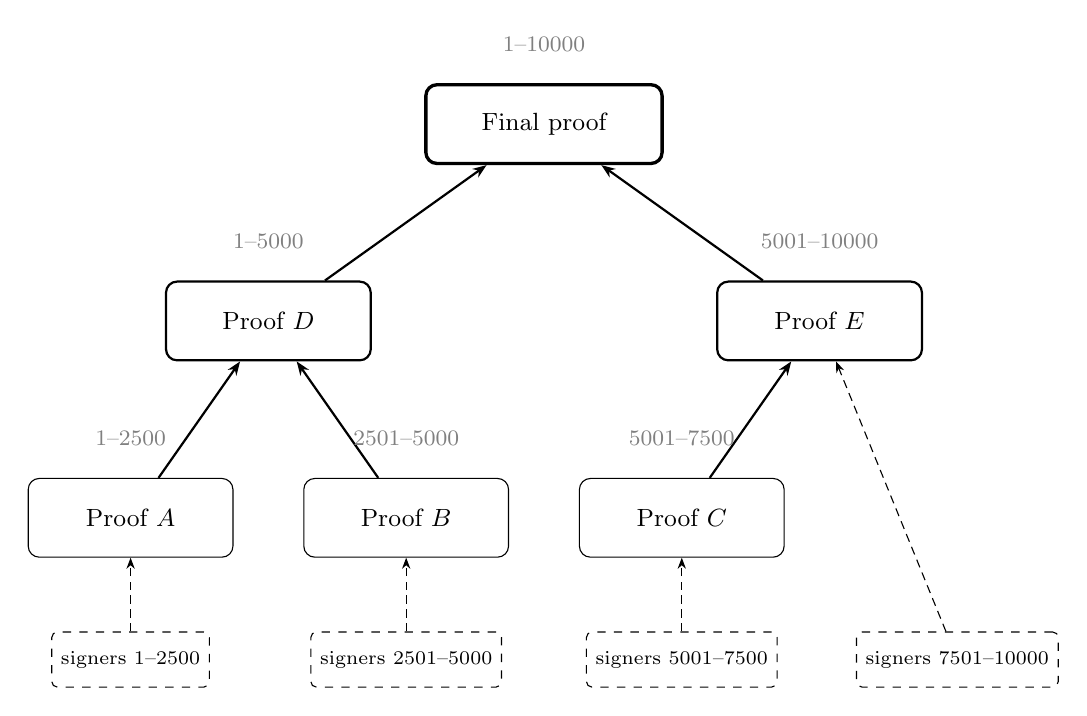
\begin{tikzpicture}[
    proof/.style={draw, rounded corners=4pt, minimum width=2.6cm, minimum height=1cm, align=center, font=\small},
    leaf/.style={proof},
    merge/.style={proof, line width=0.8pt},
    root/.style={proof, minimum width=3cm, line width=1.2pt},
    xmss/.style={draw, dashed, rounded corners=2pt, minimum width=1.6cm, minimum height=0.7cm, align=center, font=\scriptsize},
    attests/.style={font=\footnotesize, text=black!50},
    arr/.style={-{Stealth[length=5pt]}, thick},
    sigarr/.style={-{Stealth[length=4pt]}, densely dashed, thin},
]

% --- XMSS signature blocks (inputs) ---
\node[xmss] (S1) at (0, -1.8) {signers $1$--$2500$};
\node[xmss] (S2) at (3.5, -1.8) {signers $2501$--$5000$};
\node[xmss] (S3) at (7, -1.8) {signers $5001$--$7500$};
\node[xmss] (S4) at (10.5, -1.8) {signers $7501$--$10000$};

% --- Leaf proofs ---
\node[leaf] (L1) at (0, 0) {Proof $A$};
\node[leaf] (L2) at (3.5, 0) {Proof $B$};
\node[leaf] (L3) at (7, 0) {Proof $C$};

% XMSS -> leaf arrows
\draw[sigarr] (S1) -- (L1);
\draw[sigarr] (S2) -- (L2);
\draw[sigarr] (S3) -- (L3);

% --- Middle level ---
\node[merge] (M1) at (1.75, 2.5) {Proof $D$};
\node[merge] (M2) at (8.75, 2.5) {Proof $E$};

% XMSS -> E (direct group)
\draw[sigarr] (S4) -- (M2);

% Recursive arrows: leaves -> middle
\draw[arr] (L1) -- (M1);
\draw[arr] (L2) -- (M1);
\draw[arr] (L3) -- (M2);

% --- Root ---
\node[root] (R) at (5.25, 5) {Final proof};

% Recursive arrows: middle -> root
\draw[arr] (M1) -- (R);
\draw[arr] (M2) -- (R);

% --- Coverage annotations (above each proof) ---
\node[attests, above=8pt of L1] {$1\text{--}2500$};
\node[attests, above=8pt of L2] {$2501\text{--}5000$};
\node[attests, above=8pt of L3] {$5001\text{--}7500$};
\node[attests, above=8pt of M1] {$1\text{--}5000$};
\node[attests, above=8pt of M2] {$5001\text{--}10000$};
\node[attests, above=8pt of R] {$1\text{--}10000$};

\end{tikzpicture}
\caption{Example of recursive aggregation of 10000 signatures. (Note: overlapping sets of signers are possible.) }
\label{fig:recursive-aggregation}
\end{figure}


\section{VM specification}
\subsection{Field}

\fbox{KoalaBear prime: $p = 2^{31} - 2^{24} + 1$}

\vspace{3mm}

Advantages:
\begin{itemize}
    \item small field $\xrightarrow{}$ less Poseidon rounds
    \item $x \xrightarrow{} x^3$ is an automorphism of $\Fp^*$, meaning efficient S-box for Poseidon2 (in BabyBear, it's degree $7$)
    \item $< 2^{31}$ $\xrightarrow{}$ the sum of 2 field elements can be stored in an u32
\end{itemize}

The small 2-addicity (24) is not a limiting factor in WHIR, thanks to the use of an interleaved Reed Solomon code (example: with an initial folding of 7, and rate $1/2$, we can commit up to $2^{30}$ field elements).

\vspace{3mm}

\fbox{Extension field: $\Fq$, with $q = p^5$} : the degree-5 extension enables 128 bits of security in WHIR, with the Johnson bound, thanks to the latest result of \cite{proximity_gaps_rs_codes_2}.

\subsection{Memory}

\begin{itemize}
    \item Read-Only Memory
    \item Word = KoalaBear field element
    \item Memory size: $M = 2^m$ with $16 \leq m \leq 29$ ($m$ depends on the execution and is communicated at the beginning of the proof).
    \item The first $M' = 2^{m'}$ memory cells hold the "public input", on which both prover and verifier must agree.
    This enables to pass the arguments that the leanISA program receives as input (in our case: message to sign and XMSS public keys).
\end{itemize}

% \begin{figure}[h]
% \caption{Memory structure}
% \centering
% \label{memory}
% \includegraphics[scale=0.7]{images/memory.png}
% \end{figure}

\subsection{Registers}

% As in Cairo:
\begin{itemize}
    \item \fbox{\textbf{pc}: program counter} : points to the current instruction
    % \item \textbf{ap}: allocation pointer = Points to the first untouched memory cell
    \item \fbox{\textbf{fp}: frame pointer} : points to the start of the current "stack frame" in memory
\end{itemize}


Difference with Cairo: no \textbf{ap} register (allocation pointer).


\subsection{Instruction Set Architecture}

Notations:
\begin{itemize}
    \item $\alpha$, $\beta$ and $\gamma$ represent parameters of the instructions (immediate value operands)
    \item $\textbf{m}[i]$ represents the value of the memory at index $i \in \Fp$, with $i < M$ ($M$: memory size). Any out-of-bound memory access ($i \geq M$) is invalid.
    \item $\begin{cases} A \\ B \end{cases}$ When using the instruction, either $A$ or $B$ can be used, but not both simultaneously.
\end{itemize}


\subsubsection{ADD / MUL}

ADD: $\nu_a + \nu_c = \nu_b$ \hspace{3mm} and \hspace{3mm} MUL: $\nu_a \cdot \nu_c = \nu_b$ with: 

\begin{align*}
\nu_a &= 
\begin{cases}
\alpha \\
\textbf{m}[\textbf{fp} + \alpha]
\end{cases}
&
\nu_b &= 
\begin{cases}
\beta \\
\textbf{m}[\textbf{fp} + \beta]
\end{cases}
&
\nu_c &= 
\begin{cases}
\gamma \\
\textbf{m}[\textbf{fp} + \gamma]  \\
\textbf{fp} + \gamma
\end{cases}
\end{align*}


\subsubsection{DEREF}

$$
\textbf{m}[\textbf{m}[\textbf{fp} + \alpha] + \beta] = 
\begin{cases}
& \gamma \\
& \textbf{m}[\textbf{fp} + \gamma]   \\
& \textbf{fp} + \gamma

\end{cases}
$$

\subsubsection{JUMP (Conditional)}

Using the following values:

\begin{align*}
\text{condition} &= 
\begin{cases}
\alpha \\
\textbf{m}[\textbf{fp} + \alpha]
\end{cases} \in \{0, 1\}
&
\text{dest} &= 
\begin{cases}
\beta \\
\textbf{m}[\textbf{fp} + \beta]
\end{cases}
&
\text{updated\_fp} &=
\begin{cases}
\textbf{fp} + \gamma \\
\textbf{m}[\textbf{fp} + \gamma]
\end{cases}
\end{align*}

... we have the following update rules:

$$
\text{next(\textbf{pc})} =
\begin{cases}
\text{dest} & \text{if condition} = 1 \\
\text{\textbf{pc}} + 1 & \text{if condition} = 0
\end{cases}
\qquad
\text{next(\textbf{fp})} =
\begin{cases}
\text{updated\_fp} & \text{if condition} = 1 \\
\textbf{fp} & \text{if condition} = 0
\end{cases}
$$

\subsection{Precompiles}

There are two "precompile" instructions: EXTENSION\_OP and POSEIDON2, used for special computation (extension field operations and hashing). Each precompile instruction has three (potentially runtime) parameters $\nu_A$, $\nu_B$, $\nu_C$, and a compile-time value \texttt{PRECOMPILE\_DATA}.

$\nu_A$, $\nu_B$, $\nu_C$ are defined similarly to the ADD/MUL instructions, with the additional possibility of $\nu_A = \textbf{fp} + \alpha$ and $\nu_B = \textbf{fp} + \beta$, but these two must be used simultaneously (if $\nu_A$ is fp-relative, then $\nu_B$ must be fp-relative too, and vice versa).

\subsubsection{POSEIDON2}

Compression of 16 field elements (two blocks of 8) into 8 field elements.

$$
\textbf{m}[\nu_C..\nu_C + 8] = \text{Poseidon2}(\textbf{m}[\nu_A..\nu_A + 8] | \textbf{m}[\nu_B..\nu_B + 8]) + \textbf{m}[\nu_A..\nu_A + 8]
$$

\vspace{2mm}

\texttt{PRECOMPILE\_DATA} $= 1$

\subsubsection{EXTENSION\_OP}\label{extension_op_instruction}

EXTENSION\_OP enables computations of one these 3 forms in the extension field $\Fq$:

\[
\sum_{i=0}^{N-1} (a_i + b_i), \qquad
\sum_{i=0}^{N-1} (a_i \cdot b_i), \qquad
\prod_{i=0}^{N-1} (a_i b_i + (1 - a_i)(1 - b_i))
\]

\vspace{2mm}

\underbar{Details}

\vspace{2mm}

For $i = 0, \ldots, N-1$, define:
$$b_i = \textbf{m}[\nu_B + 5i \,..\, \nu_B + 5i + 5] \in \Fq$$
and $a_i$ depends on the mode:
\begin{itemize}
    \item \textbf{BE mode} (\texttt{is\_be} $= 1$): $a_i = \textbf{m}[\nu_A + i] \in \Fp$, embedded in $\Fq$ as $[a_i, 0, 0, 0, 0]$.
    \item \textbf{EE mode} (\texttt{is\_be} $= 0$): $a_i = \textbf{m}[\nu_A + 5i \,..\, \nu_A + 5i + 5] \in \Fq$.
\end{itemize}

(Chunks of 5 field elements $\textbf{m}[x..x+5]$ are interpreted as an extension field element ($\Fq = {\mathbb F_{p^5}}$)).

\vspace{2mm}

Three operation modes determine both the per-element computation $e_i$ and the accumulation method:
\begin{itemize}
    \item \textbf{ADD}: $e_i = a_i + b_i$, \quad $\text{result} = \displaystyle\sum_{i=0}^{N-1} e_i$ \hfill (additive accumulation)
    \item \textbf{MUL}: $e_i = a_i \cdot b_i$, \quad $\text{result} = \displaystyle\sum_{i=0}^{N-1} e_i$ \hfill (additive accumulation = dot product)
    \item \textbf{POLY\_EQ}: $e_i = a_i b_i + (1 - a_i)(1 - b_i)$, \quad $\text{result} = \displaystyle\prod_{i=0}^{N-1} e_i$ \hfill (multiplicative)
\end{itemize}

The result is stored at $\textbf{m}[\nu_C \,..\, \nu_C + 5] \in \Fq$.

\vspace{2mm}

\texttt{PRECOMPILE\_DATA} encodes the mode, the operand type, and the length:
$$\texttt{PRECOMPILE\_DATA} = 2 \cdot \texttt{is\_be} + 4 \cdot \texttt{flag\_add} + 8 \cdot \texttt{flag\_mul} + 16 \cdot \texttt{flag\_poly\_eq} + 32 \cdot N$$
where exactly one of \texttt{flag\_add}, \texttt{flag\_mul}, \texttt{flag\_poly\_eq} is 1, and $N \geq 1$. This encoding is injective and always disjoint from Poseidon ($= 1$) and no-precompile ($= 0$).


\subsection{ISA programming}

\subsubsection{Functions}

\begin{enumerate}
    \item Each function has a deterministic memory footprint: the length of the continuous frame in memory that is allocated for each of the its calls.
    \item At runtime, each time we call our function, we receive via a memory cell a hint pointing to a free range of memory. We then store the current values of \textbf{pc} / \textbf{fp} at the start of this newly allocated frame, alongside the function's arguments, we can then jump, to enter the function bytecode, and modify \textbf{fp} with the hinted value. The intuition here is that the verifier does not care where the new memory frame will be placed (we use a read-only memory, so we cannot overwrite previous frames). In practice, the prover that runs the program would need to keep the value of the allocation pointer "ap", in order to adequately allocate new memory frames, but there is no need to keep track of it from the versifier's perspective.
\end{enumerate}


\begin{figure}[h]
\caption{Memory layout of a function call}
\centering
\includegraphics[scale=0.4]{images/memory_layout.png}
\end{figure}

\subsubsection{Loops}\label{loops}

We suggest to unroll loops when the number of iterations is low, and known at compile time.
The remaining loops are transformed into recursive functions (by the leanISA compiler).

\subsubsection{Range checks}

\fbox{It's possible to check that a given memory cell is smaller than some value $t$ (for $t \leq 2^{16})$ in 3 cycles.}

We denote by \textbf{m}[\textbf{fp} + $x$] the memory cell for which we want to ensure \textbf{m}[\textbf{fp} + $x$] $< t$.
We also denote by \textbf{m}[\textbf{fp} + $i$], \textbf{m}[\textbf{fp} + $j$] and \textbf{m}[\textbf{fp} + $k$] 3 auxiliary memory cells (that have not been used yet).
\begin{enumerate}
    \item \textbf{m}[\textbf{m}[\textbf{fp} + $x$]] = \textbf{m}[\textbf{fp} + $i$] (using DEREF, this ensures \textbf{m}[\textbf{fp} + $x$] $ < M$, the memory size)
    \item \textbf{m}[\textbf{m}[\textbf{fp} + $x$]] + \textbf{m}[\textbf{fp} + $j$] = (t-1) (using ADD)
        \item \textbf{m}[\textbf{m}[\textbf{fp} + $j$]] = \textbf{m}[\textbf{fp} + $k$] (using DEREF, this ensures $t - 1 - $ \textbf{m}[\textbf{fp} + $x$] $ < M$)
\end{enumerate}

Given $t \leq 2^{16} \leq M$, \textbf{m}[\textbf{fp} + $x$] $ < M$, $t - 1 - $ \textbf{m}[\textbf{fp} + $x$] $< M$, and $M \leq 2^{29} < p / 2$, we have: \textbf{m}[\textbf{fp} + $x$] $ < t$.

Note: From the point of view of the prover running the program, some hints are necessary (filling the values of \textbf{m}[\textbf{fp} + $i$] and \textbf{m}[\textbf{fp} + $k$] must be done at end of execution).

This idea was pointed out by D. Khovratovich, and is an unplanned use of the DEREF instruction.

\begin{exmp}
	Let's say we want to write a function with 2 arguments $x = \textbf{m}$[\textbf{fp} + 2] and $y = \textbf{m}$[\textbf{fp} + 3] ($\textbf{m}$[\textbf{fp} + 0] and $\textbf{m}$[\textbf{fp} + 1] are used, by convention, to store the caller's \textbf{pc} and \textbf{fp}, to return to the previous context at the end of the function), which perform the following:
	
	\begin{enumerate}
		\item assert(x $<$ 10)
		\item z := x*y + 100
		\item assert(z $<$ 1000)
	\end{enumerate}
	
	Which can be compiled to:
	
	\begin{enumerate}
		\item \textbf{m}[\textbf{fp} + 4] = \textbf{m}[$\big[$\textbf{fp} + 2$\big]$] // check that $x$ is "small"
		\item \textbf{m}[\textbf{fp} + 2] + \textbf{m}[\textbf{fp} + 5] = 9 // compute $9 - x$
		\item \textbf{m}[\textbf{fp} + 6] = \textbf{m}[$\big[$\textbf{fp} + 5$\big]$] // check that $9 - x$ is "small"
		\item \textbf{m}[\textbf{fp} + 7] = \textbf{m}[\textbf{fp} + 2] * \textbf{m}[\textbf{fp} + 3] // compute $x.y$
		\item \textbf{m}[\textbf{fp} + 8] = \textbf{m}[\textbf{fp} + 7] + 100 // compute $z = x.y + 100$
		\item \textbf{m}[\textbf{fp} + 9] = \textbf{m}[$\big[$\textbf{fp} + 8$\big]$] // check that $z$ is "small"
		\item \textbf{m}[\textbf{fp} + 8] + \textbf{m}[\textbf{fp} + 10] = 999 // compute $999 - z$
		\item \textbf{m}[\textbf{fp} + 11] = \textbf{m}[$\big[$\textbf{fp} + 10$\big]$] // check that $999 - z$ is "small"
		\item JUMP with next(\textbf{pc}) = \textbf{m}[\textbf{fp} + 0], next(\textbf{fp}) = \textbf{m}[\textbf{fp} + 1], condition = 1 // return
	\end{enumerate}
	
	 
\end{exmp}


\subsubsection{Switch statements}

Suppose we want a different logic depending on the value $x$ of a given memory cell, where $x$ is known to be $< k$ (if the value $x$ comes from a "hint", don't forget to range-check it).

Each of the $k$ different value leads to a different branch at runtime, represented by a block of code. We want to jump to the correct block of code depending on $x$.
One efficient implementation consists in placing our blocks of code at regular intervals, and to jump to a $a+ b.x$, where $a$ is the offset of the first block of code (in case $x = 0$), and $b$ is the distance between two consecutive blocks.
\newline
\newline
Example: During XMSS verification, for each of the $v$ chains, we need to hash a pre-image, a number of times depending on the encoding, but known to be $< w$. Here $k = w$, and the $i-th$ block of code we could jump to will execute $i$ times the hash function (unrolled loop).

\section{Proving system}\label{sec:proving}

\subsection{Table sizes}\label{sec:table-sizes}

Each table has a maximum number of rows (as a power of two):

\begin{center}
\begin{tabular}{lc}
\toprule
Table & Max rows \\
\midrule
Execution & $2^{25}$ \\
Extension op & $2^{20}$ \\
Poseidon & $2^{21}$ \\
\bottomrule
\end{tabular}
\end{center}

Tables are padded to the next power of two (with a minimum of $2^{8}$ rows). These bounds are critical for soundness: they ensure that logup multiplicities cannot overflow modulo $p$.

\subsection{Arithmetic Intermediate Representation (AIR)}\label{sec:air-eval}

If a table has $n$ columns, a transition constraint is a multivariate polynomial $C(x_1, \dots, x_n, y_1, \dots, y_n)$ in $2n$ variables, where $(x_1, \dots, x_n)$ represents the current row and $(y_1, \dots, y_n)$ represents the next row. Each table defines a set of such constraints, all of which must evaluate to zero on every pair of consecutive rows. For a table with $H$ rows (indexed $0, \dots, H-1$), the constraints are evaluated on $(H-1) + 1 = H$ pairs:
\begin{itemize}
    \item $H - 1$ consecutive pairs: $(\text{row}_i, \text{row}_{i+1})$ for $i = 0, \dots, H-2$
    \item 1 \textbf{wrapping pair}: $(\text{row}_{H-1}, \text{row}_{H-1})$ --- the last row is paired with itself
\end{itemize}

The wrapping pair means that on the last row, $\text{next}(x) = x$ for every column $x$.

\vspace{3mm}

TODO: describe how to prove AIR via sumcheck.

\subsection{Execution table}


\subsubsection{Commitment}

\fbox{At each cycle, we commit to 20 (base) field elements:}

\begin{itemize}
    \item \textbf{pc} (program counter)
    \item \textbf{fp} (frame pointer)
    % \item jump (non zero when a jump occurs)
    \item $\text{addr}_A$, $\text{addr}_B$, $\text{addr}_C$
    \item $\text{value}_A = \textbf{m}[\text{addr}_A]$, $\text{value}_B = \textbf{m}[\text{addr}_B]$, $\text{value}_C = \textbf{m}[\text{addr}_C]$
    \item 12 field elements describing the instruction being executed (see below)
\end{itemize}


\subsubsection{Instruction Encoding}

Each instruction is described by 12 field elements ($\Fp$):

\begin{itemize}
    \item 3 operands: $\text{operand}_A$, $\text{operand}_B$, $\text{operand}_C$
    \item 5 flags ($\in \{0, 1\}$): $\text{flag}_A$, $\text{flag}_B$, $\text{flag}_C$, $\text{flag}^{C}_\textbf{fp}$, $\text{flag}^{AB}_\textbf{fp}$
    \item 3 opcode flags: MUL ($\in \{0, 1\}$), JUMP ($\in \{0, 1\}$), AUX ($\in \{0, 1, 2\}$) (AUX handles both ADD and DEREF)
    \item PRECOMPILE\_DATA
\end{itemize}

$\text{flag}^{AB}_\textbf{fp}$ is only used by precompile instructions; for ADD, MUL, DEREF, and JUMP it is always 0.


\subsubsection{AIR transition constraints}

\fbox{We use transition constraints of degree 5.}

\vspace{5mm}

We define the following values:
\begin{itemize}
    \item $\nu_A = \text{flag}_A \cdot \text{operand}_A + (1 - \text{flag}_A - \text{flag}^{AB}_\textbf{fp}) \cdot \text{value}_A + \text{flag}^{AB}_\textbf{fp} \cdot (\textbf{fp} + \alpha)$ 
    \item $\nu_B = \text{flag}_B \cdot \text{operand}_B + (1 - \text{flag}_B - \text{flag}^{AB}_\textbf{fp}) \cdot \text{value}_B + \text{flag}^{AB}_\textbf{fp} \cdot (\textbf{fp} + \beta)$
    \item $\nu_C = \text{flag}_C \cdot \text{operand}_C + (1 - \text{flag}_C - \text{flag}_\textbf{fp}) \cdot \text{value}_C + \text{flag}_\textbf{fp} \cdot (\textbf{fp} + \gamma)$
\end{itemize}


With the associated constraints:
\begin{itemize}
    \item $(1 - \text{flag}_A - \text{flag}^{AB}_\textbf{fp}) \cdot (\text{address}_A - (\textbf{fp} + \text{operand}_A)) = 0$
    \item $(1 - \text{flag}_B - \text{flag}^{AB}_\textbf{fp}) \cdot (\text{address}_B - (\textbf{fp} + \text{operand}_B)) = 0$
    \item $(1 - \text{flag}_C - \text{flag}^{C}_\textbf{fp}) \cdot (\text{address}_C - (\textbf{fp} + \text{operand}_C)) = 0$
\end{itemize}

\vspace{3mm}\centerline{\rule{10cm}{0.4pt}}\vspace{5mm}

Let $P_0, P_1, P_2$ be the Lagrange basis polynomials at points $0, 1, 2$. Explicitely:

$$P_0(x) = (x-1)\cdot(x-2) / 2 \hspace{10mm} P_1(x) = x \cdot (2-x) \hspace{10mm} P_2(x) = x \cdot (x-1) / 2$$

We define the following values:

\begin{itemize}
    \item ADD = $P_1(\text{AUX})$
    \item DEREF = $P_2(\text{AUX})$
    \item IS\_PRECOMPILE = $1 - (\text{ADD} + \text{MUL} + \text{DEREF} + \text{JUMP})$
\end{itemize}

IS\_PRECOMPILE is used a "bus selector" (see \ref{buses}).

\vspace{3mm}\centerline{\rule{10cm}{0.4pt}}\vspace{5mm}

PRECOMPILE\_DATA encodes the precompile being called, and the parameters of the call:
\begin{itemize}
    \item No precompile $\rightarrow$ PRECOMPILE\_DATA $= 0$
    \item Poseidon precompile $\rightarrow$ PRECOMPILE\_DATA $= 1$
    \item Extension op precompile $\rightarrow$ PRECOMPILE\_DATA $= 2 \cdot \texttt{is\_be} + 4 \cdot \texttt{flag\_add} + 8 \cdot \texttt{flag\_mul} + 16 \cdot \texttt{flag\_poly\_eq} + 32 \cdot N$ \hfill ($N$ = length)
\end{itemize}

\vspace{3mm}\centerline{\rule{10cm}{0.4pt}}\vspace{5mm}

For addition, set AUX $= 1$.
\begin{itemize}
    \item $\text{ADD} \cdot(\nu_B - (\nu_A + \nu_C)) = 0$
\end{itemize}


\vspace{3mm}\centerline{\rule{10cm}{0.4pt}}\vspace{5mm}

For multiplication, set MUL $= 1$.
\begin{itemize}
    \item $\text{MUL} \cdot(\nu_B - \nu_A \cdot \nu_C) = 0$
\end{itemize}

\vspace{3mm}\centerline{\rule{10cm}{0.4pt}}\vspace{5mm}

For DEREF instructions, set AUX $= 2$, $\text{flag}_A = 0$, $\text{flag}_B = 1$ and $\text{flag}_C$ / $\text{flag}^{C}_\textbf{fp}$ according to whether the third operand is an immediate value, a memory read, or fp-relative.

The relation $\textbf{m}[\textbf{m}[\textbf{fp} + \alpha] + \beta] = \nu_C$ is then captured by:

\begin{itemize}
    \item $\text{DEREF} \cdot (\text{addr}_B - (\text{value}_A + \text{operand}_B)) = 0$
    \item $\text{DEREF} \cdot (\text{value}_B - \nu_C) = 0$
\end{itemize}

\vspace{3mm}\centerline{\rule{10cm}{0.4pt}}\vspace{5mm}

For (conditional) jumps, set JUMP = 1, with the following constraints, using $J = \text{JUMP} \cdot \nu_A$:
\begin{itemize}
    \item $J \cdot (1 - \nu_A) = 0$
    \item $J \cdot ( \text{next(\textbf{pc})} - \nu_B) = 0$
    \item $J \cdot ( \text{next(fp)} - \nu_C) = 0$
    \item $(1 - J) \cdot ( \text{next(\textbf{pc})} - (\text{\textbf{pc}} + 1)) = 0$
    \item $(1 - J) \cdot (\text{next(fp)} - \textbf{fp}) = 0$
\end{itemize}

Note: the constraint $J \cdot (1 - \nu_A) = 0$ could be removed, as long as it's correctly enforced in the bytecode.

\vspace{3mm}

TODO: Verify and (formally) prove soundness.

\subsection{Poseidon table}

TODO

\subsection{Extension op table}

See \ref{extension_op_instruction} for the instruction specification.

\subsubsection{Trace layout}

Each extension field operation occupies $N$ consecutive rows (one row per element pair). Within a group, rows are ordered from first element to last, but the \texttt{computation} column accumulates backward: the first row holds the full result, the last row holds only the final element's value. Padding rows have all operation flags set to 0 and $\texttt{start} = 1$, $\texttt{len} = 1$.

\vspace{3mm}

\noindent\resizebox{\textwidth}{!}{%
\begin{tabular}{cccccccccc|cccc|c}
\toprule
\multicolumn{10}{c|}{Base field columns ($\Fp$)} & \multicolumn{4}{c|}{Extension field columns ($\Fq$)} & \\
\texttt{start} & $\texttt{f}_\texttt{add}$ & $\texttt{f}_\texttt{mul}$ & $\texttt{f}_\texttt{peq}$ & \texttt{len} & $\text{idx}_A$ & $\text{idx}_B$ & $\text{idx}_R$ & \texttt{is\_be} & $v_{A,\Fp}$ & $v_{A,\Fq}$ & $v_B$ & \texttt{comp} & \texttt{res} & \texttt{aux} \\
\midrule
\multicolumn{15}{l}{\textit{MUL, BE, $N\!=\!4$ ($\nu_A\!=\!90$, $\nu_B\!=\!211$, $\nu_C\!=\!74$): \quad $\texttt{res} = \sum_{i=0}^{3} \textbf{m}[90\!+\!i] \cdot \textbf{m}[211\!+\!5i..216\!+\!5i]$}} \\[2pt]
1 & 0 & 1 & 0 & 4 & 90  & 211 & 74 & 1 & $\textbf{m}[90]$  & $\textbf{m}[90..95]$  & $\textbf{m}[211..216]$ & $e_0\!+\!e_1\!+\!e_2\!+\!e_3$ & $\textbf{m}[74..79]$ & 138 \\
0 & 0 & 1 & 0 & 3 & 91  & 216 & 74 & 1 & $\textbf{m}[91]$  & $\textbf{m}[91..96]$  & $\textbf{m}[216..221]$ & $e_1\!+\!e_2\!+\!e_3$       & $\textbf{m}[74..79]$ & 106 \\
0 & 0 & 1 & 0 & 2 & 92  & 221 & 74 & 1 & $\textbf{m}[92]$  & $\textbf{m}[92..97]$  & $\textbf{m}[221..226]$ & $e_2\!+\!e_3$               & $\textbf{m}[74..79]$ & 74 \\
0 & 0 & 1 & 0 & 1 & 93  & 226 & 74 & 1 & $\textbf{m}[93]$  & $\textbf{m}[93..98]$  & $\textbf{m}[226..231]$ & $e_3$                       & $\textbf{m}[74..79]$ & 42  \\
\midrule
\multicolumn{15}{l}{\textit{ADD, EE, $N\!=\!3$ ($\nu_A\!=\!400$, $\nu_B\!=\!500$, $\nu_C\!=\!300$): \quad $\texttt{res} = \sum_{i=0}^{2} (\textbf{m}[400\!+\!5i..405\!+\!5i] + \textbf{m}[500\!+\!5i..505\!+\!5i])$}} \\[2pt]
1 & 1 & 0 & 0 & 3 & 400 & 500 & 300 & 0 & $\textbf{m}[400]$ & $\textbf{m}[400..405]$ & $\textbf{m}[500..505]$ & $e_0\!+\!e_1\!+\!e_2$ & $\textbf{m}[300..305]$ & 100 \\
0 & 1 & 0 & 0 & 2 & 405 & 505 & 300 & 0 & $\textbf{m}[405]$ & $\textbf{m}[405..410]$ & $\textbf{m}[505..510]$ & $e_1\!+\!e_2$         & $\textbf{m}[300..305]$ & 68 \\
0 & 1 & 0 & 0 & 1 & 410 & 510 & 300 & 0 & $\textbf{m}[410]$ & $\textbf{m}[410..415]$ & $\textbf{m}[510..515]$ & $e_2$                 & $\textbf{m}[300..305]$ & 36 \\
\midrule
\multicolumn{15}{l}{\textit{POLY\_EQ, EE, $N\!=\!3$ ($\nu_A\!=\!600$, $\nu_B\!=\!700$, $\nu_C\!=\!800$): \quad $\texttt{res} = \prod_{i=0}^{2} [a_i b_i + (1\!-\!a_i)(1\!-\!b_i)]$}} \\[2pt]
1 & 0 & 0 & 1 & 3 & 600 & 700 & 800 & 0 & $\textbf{m}[600]$ & $\textbf{m}[600..605]$ & $\textbf{m}[700..705]$ & $e_0 \cdot e_1 \cdot e_2$ & $\textbf{m}[800..805]$ & 112 \\
0 & 0 & 0 & 1 & 2 & 605 & 705 & 800 & 0 & $\textbf{m}[605]$ & $\textbf{m}[605..610]$ & $\textbf{m}[705..710]$ & $e_1 \cdot e_2$           & $\textbf{m}[800..805]$ & 80 \\
0 & 0 & 0 & 1 & 1 & 610 & 710 & 800 & 0 & $\textbf{m}[610]$ & $\textbf{m}[610..615]$ & $\textbf{m}[710..715]$ & $e_2$                     & $\textbf{m}[800..805]$ & 48 \\
\midrule
\multicolumn{15}{l}{\textit{Padding row}} \\[2pt]
1 & 0 & 0 & 0 & 1 & 0   & 0   & 0  & 0 & $\textbf{m}[0]$ & $\textbf{m}[0..5]$ & $\textbf{m}[0..5]$ & 0 & $\textbf{m}[0..5]$ & 32 \\
\bottomrule
\end{tabular}%
}

\vspace{3mm}

Notes: $e_i$ denotes the per-element result (virtual, not a committed column). Both lookups $v_{A,\Fp} = \textbf{m}[\text{idx}_A]$ and $v_{A,\Fq} = \textbf{m}[\text{idx}_A..+5]$ are performed unconditionally; in BE mode only $v_{A,\Fp}$ is used, in EE mode only $v_{A,\Fq}$ is used. \texttt{aux} is a non-committed bus fingerprinting column, equal to $2 \cdot \texttt{is\_be} + 4 \cdot \texttt{flag\_add} + 8 \cdot \texttt{flag\_mul} + 16 \cdot \texttt{flag\_poly\_eq} + 32 \cdot \texttt{len}$ on each row. The bus selector is the virtual column $\texttt{activation\_flag} = \texttt{start} \cdot \texttt{active}$ (not shown; equals \texttt{start} on active rows, 0 on padding).

\subsubsection{Columns}

\fbox{10 base field columns + 4 extension field columns = 30 $\Fp$-columns.}

\vspace{3mm}

\textbf{Base field columns ($\Fp$, 10 AIR + 2 non-AIR):}
\begin{itemize}
    \item \texttt{is\_be} $\in \{0,1\}$: mode flag (1: base $\times$ extension, 0: xextension $\times$ extension)
    \item \texttt{start} $\in \{0,1\}$: group boundary (1 on first row of each group and on padding, 0 elsewhere)
    \item $\texttt{flag\_add}$, $\texttt{flag\_mul}$, $\texttt{flag\_poly\_eq}$ $\in \{0,1\}$: operation selectors (exactly one is 1 on active rows, all 0 on padding)
    \item \texttt{len}: countdown from $N$ to 1 within each group (1 on padding)
    \item $\text{idx}_A$: memory address (increments by 1 in BE, by 5 in EE within a group)
    \item $\text{idx}_B$: memory address (increments by 5 within a group)
    \item $\text{idx}_R$: memory address for the result (constant within a group)
    \item $v_{A,\Fp}$: base field value $\textbf{m}[\text{idx}_A]$ (used in BE mode)
\end{itemize}

\textbf{Extension field columns ($\Fq$, 4 AIR):}
\begin{itemize}
    \item $v_{A,\Fq}$: extension field value $\textbf{m}[\text{idx}_A .. \text{idx}_A + 5]$ (used in EE mode)
    \item $v_B$: extension field value $\textbf{m}[\text{idx}_B .. \text{idx}_B + 5]$
    \item \texttt{res}: result value $\textbf{m}[\text{idx}_R .. \text{idx}_R + 5]$ (same on every row of a group)
    \item \texttt{computation}: running accumulation; equals \texttt{res} on \texttt{start} rows
\end{itemize}

\textbf{Non-committed columns} (used for bus interaction):
\begin{itemize}
    \item $\texttt{activation\_flag} = \texttt{start} \cdot \texttt{active}$: bus selector (1 on first row of each active group, 0 elsewhere)
    \item \texttt{aux} $= 2 \cdot \texttt{is\_be} + 4 \cdot \texttt{flag\_add} + 8 \cdot \texttt{flag\_mul} + 16 \cdot \texttt{flag\_poly\_eq} + 32 \cdot \texttt{len}$
\end{itemize}

\subsubsection{Memory lookups}
\begin{itemize}
    \item $v_{A,\Fp} = \textbf{m}[\text{idx}_A]$ \hfill
    \item $v_{A,\Fq} = \textbf{m}[\text{idx}_A..+5]$ \hfill
    \item $v_B = \textbf{m}[\text{idx}_B..+5]$
    \item $\texttt{res} = \textbf{m}[\text{idx}_R..+5]$
\end{itemize}

\subsubsection{Bus interaction}
On rows where $\texttt{activation\_flag} = 1$ (i.e.\ $\texttt{start} = 1$ and $\texttt{active} = 1$), the table \textsc{Pull}s $(\texttt{aux}, \text{idx}_A, \text{idx}_B, \text{idx}_R)$ from the precompile bus. The execution table \textsc{Push}es a matching tuple for each EXTENSION\_OP instruction.


The $\texttt{aux}$ encoding ensures both the mode and the length are bound to the bus data. Since $\texttt{is\_be}$, $\texttt{flag\_add}$, $\texttt{flag\_mul}$, and $\texttt{flag\_poly\_eq}$ are constrained to be boolean, and since the length is constrained to be $\leq 2^{20}$ (by Lemma~\ref{lem:len-bound}), no overflow can occur modulo $p$ and the $\texttt{aux}$ value is unique for each combination of parameters, which enforces that all values of PRECOMPILE\_DATA sent by the execution table are correctly received by the extension\_op table.


\subsubsection{AIR constraints}

\fbox{Degree 6.}

\vspace{2mm}

\textbf{Value selection:} Define:
$$v_A = \texttt{is\_be} \cdot v_{A,\Fp} + (1 - \texttt{is\_be}) \cdot v_{A,\Fq} \;\in \Fq$$

Let $\texttt{active} = \texttt{flag\_add} + \texttt{flag\_mul} + \texttt{flag\_poly\_eq}$ (1 on active rows, 0 on padding), and define the per-element results (virtual):
\begin{align*}
    e_\text{add} &= v_A + v_B \\
    e_\text{mul} &= v_A \cdot v_B \\
    e_\text{peq} &= v_A \cdot v_B + (1 - v_A)(1 - v_B)
\end{align*}

Let $\texttt{comp\_tail} = \text{next}(\texttt{comp}) \cdot (1 - \text{next}(\texttt{start}))$ (zero when the next row is a new group).

\vspace{2mm}

\textbf{Boolean constraints:}
\begin{enumerate}
    \item $\texttt{is\_be} \cdot (1 - \texttt{is\_be}) = 0$
    \item $\texttt{start} \cdot (1 - \texttt{start}) = 0$
    \item $\texttt{flag\_add} \cdot (1 - \texttt{flag\_add}) = 0$
    \item $\texttt{flag\_mul} \cdot (1 - \texttt{flag\_mul}) = 0$
    \item $\texttt{flag\_poly\_eq} \cdot (1 - \texttt{flag\_poly\_eq}) = 0$
\end{enumerate}

\textbf{Accumulation constraint:}
\begin{enumerate}
    \setcounter{enumi}{5}
    \item $\texttt{f}_\texttt{add} \cdot (\texttt{comp} - e_\text{add} - \texttt{comp\_tail}) = 0$ \hfill (additive ADD)
    \item $\texttt{f}_\texttt{mul} \cdot (\texttt{comp} - e_\text{mul} - \texttt{comp\_tail}) = 0$ \hfill (additive MUL)
    \item $\texttt{f}_\texttt{peq} \cdot (\texttt{comp} - e_\text{peq} \cdot (\texttt{comp\_tail} + \text{next}(\texttt{start}))) = 0$ \hfill (multiplicative POLY\_EQ)
\end{enumerate}

\vspace{2mm}

\textbf{Result constraint:}
\begin{enumerate}
    \setcounter{enumi}{8}
    \item $\texttt{start} \cdot (\texttt{comp} - \texttt{res}) = 0$ \hfill (on start rows, computation equals result)
\end{enumerate}

\textbf{Intra-group consistency:}
\begin{enumerate}
    \setcounter{enumi}{9}
    \item $(1 - \text{next}(\texttt{start})) \cdot (\texttt{len} - \text{next}(\texttt{len}) - 1) = 0$ \hfill (len countdown)
    \item $(1 - \text{next}(\texttt{start})) \cdot (\texttt{is\_be} - \text{next}(\texttt{is\_be})) = 0$ \hfill (mode consistent)
    \item $(1 - \text{next}(\texttt{start})) \cdot (\texttt{f}_\texttt{add} - \text{next}(\texttt{f}_\texttt{add})) = 0$
    \item $(1 - \text{next}(\texttt{start})) \cdot (\texttt{f}_\texttt{mul} - \text{next}(\texttt{f}_\texttt{mul})) = 0$
    \item $(1 - \text{next}(\texttt{start})) \cdot (\texttt{f}_\texttt{peq} - \text{next}(\texttt{f}_\texttt{peq})) = 0$
    \item $(1 - \text{next}(\texttt{start})) \cdot (\text{next}(\text{idx}_A) - \text{idx}_A - (\texttt{is\_be} + (1 - \texttt{is\_be}) \cdot 5)) = 0$
    \item $(1 - \text{next}(\texttt{start})) \cdot (\text{next}(\text{idx}_B) - \text{idx}_B - 5) = 0$
\end{enumerate}

\textbf{Boundary:}
\begin{enumerate}
    \setcounter{enumi}{16}
    \item $\text{next}(\texttt{start}) \cdot (\texttt{len} - 1) = 0$ \hfill (when next row is a group start, current len must be 1)
\end{enumerate}

\vspace{5mm}

\begin{lemma}\label{lem:len-bound}
On every row $r$ of the dot product table, $\texttt{len}_r \leq H - r$ (as an integer in $\{0, \dots, p-1\}$), where $H \leq 2^{21}$ is the table height. In particular, $\texttt{len}_r \leq H$.
\end{lemma}

\begin{proof}
By backward induction on $r$, from $r = H - 1$ down to $r = 0$.

\vspace{2mm}

\textbf{Base case ($r = H - 1$):} On the wrapping pair (row $H\!-\!1$ paired with itself, see Section~\ref{sec:air-eval}), $\text{next}(x) = x$ for every column $x$. Constraint~10 becomes $(1 - \texttt{start}) \cdot (\texttt{len} - \texttt{len} - 1) = -(1 - \texttt{start}) = 0$, forcing $\texttt{start}_{H-1} = 1$. Then constraint~17 becomes $1 \cdot (\texttt{len} - 1) = 0$, giving $\texttt{len}_{H-1} = 1 = H - (H-1)$.

\vspace{2mm}

\textbf{Inductive step ($r < H - 1$):} Assume $\texttt{len}_s \leq H - s$ for all $s > r$. The pair (row $r$, row $r\!+\!1$) gives two cases depending on $\texttt{start}_{r+1} \in \{0,1\}$ (constraint~2):

\begin{itemize}
    \item If $\texttt{start}_{r+1} = 1$: constraint~17 gives $1 \cdot (\texttt{len}_r - 1) = 0$, so $\texttt{len}_r = 1 \leq H - r$.
    \item If $\texttt{start}_{r+1} = 0$: constraint~10 gives $(1 - 0) \cdot (\texttt{len}_r - \texttt{len}_{r+1} - 1) = 0$, so $\texttt{len}_r = \texttt{len}_{r+1} + 1$ in $\Fp$. By induction, $\texttt{len}_{r+1} \leq H - (r+1)$, so $\texttt{len}_{r+1} + 1 \leq H - r$. Since $H - r \leq H \leq 2^{21} < p$, the addition does not overflow modulo $p$, so $\texttt{len}_r = \texttt{len}_{r+1} + 1 \leq H - r$ as integers.
\end{itemize}
\end{proof}

\vspace{3mm}

TODO: Verify and (formally) prove soundness.

\subsection{Data flow between tables / memory}


\begin{lemma}
    Let $a_0, a_1, \ldots, a_{n-1}$ be pairwise distinct poles in $\Fq$, and let $m_0, m_1, \ldots, m_{n-1}$ be an associated list of multiplicities in $\{0, 1, \dots, p - 1\}$. Consider the rational function:
$$P(X) = \sum_{i=0}^{n-1} \frac{m_i}{X - a_i}$$

Except with probability $n/q$, if $P(\alpha) = 0$ for a random $\alpha \in \Fq$, then all multiplicities $m_i = 0$.

\end{lemma}

\subsubsection{Indexed Lookup into Memory}

We use logup \cite{logup}, in its indexed form, to allow tables to perform lookups into the read-only memory.


\vspace{3mm}

Let $\mathcal{T}$ denote the set of all tables in the system. For each table $T \in \mathcal{T}$ with $H_T$ rows, let $n_T$ denote the number of memory lookups. Each lookup $i < n_T$ consists of an \textbf{index column} $\text{col}_{\text{index},T,i}$ and a \textbf{value column} $\text{col}_{\text{val},T,i}$.

\vspace{3mm}

The rule to enforce is the following:
$$\forall T \in \mathcal{T}, \forall i < n_T, \forall j < H_T: \quad \text{col}_{\text{val},T,i}(j) = \textbf{m}[\text{col}_{\text{index},T,i}(j)]$$

Implicitly, we must also have $\text{col}_{\text{index},T,i}(j) < M$ (the memory size).

\vspace{3mm}

The prover initially commits to a multilinear polynomial $\textit{acc}$, having the same size as the memory, such that (in the honest case) for every $k < M$:
$$\textit{acc}[k] = \sum_{T \in \mathcal{T}} \sum_{i < n_T} \left| \{ j < H_T : \text{col}_{\text{index},T,i}(j) = k \} \right|$$
i.e., $\textit{acc}[k]$ represents the total number of times address $k$ is accessed by the lookups across all tables.

\vspace{3mm}

The verifier sends a random challenge $\alpha \in \Fq$ (TODO quantify soundness error). Let $N = \sum_{T \in \mathcal{T}} n_T \cdot H_T$ be the total number of memory lookups. Assuming $N < p$ (to avoid overflow), the indexed lookup into memory is valid, except with probability $(N + M)/q$, if for a randomly sampled $X \in \Fq$:

$$\sum_{T \in \mathcal{T}} \sum_{i<n_T} \sum_{j<H_T} \frac{1}{X - (\text{col}_{\text{index},T,i}(j) + \alpha \cdot \text{col}_{\text{val},T,i}(j))} = \sum_{k<M} \frac{\textit{acc}(k)}{X - (k + \alpha \cdot \textbf{m}[k])}$$

This can be computed via GKR, as introduced in \cite{logup_gkr}.

\subsubsection{Precompile bus: Data flow between tables}\label{buses}

See OpenVM \cite{openvm}, definition 2.2.2, for more details.

At each cycle when IS\_PRECOMPILE = 1, the execution table \textsc{Push}es $$\sigma = (\text{PRECOMPILE\_DATA}, \nu_A, \nu_B, \nu_C)$$ to the "precompile bus".

In case of Poseidon call, PRECOMPILE\_DATA = 1 and $\nu_A$, $\nu_B$, $\nu_C$ represent the left input address, the right input address, and the output address (3 pointers to a chunk of 8 field elements in memory).

In case of extension op call, PRECOMPILE\_DATA $= 2 \cdot \texttt{is\_be} + 4 \cdot \texttt{flag\_add} + 8 \cdot \texttt{flag\_mul} + 16 \cdot \texttt{flag\_poly\_eq} + 32 \cdot N$ encodes the mode, the operation, and the length $N$, and $\nu_A$, $\nu_B$, $\nu_C$ represent the starting address of the first operand, the starting address of the second operand, and the address of the result.

Each such tuple $\sigma$ (counting multiplicity) must be \textsc{Pulled} by one of the precompile tables. Given that the Poseidon table only pulls tuples with PRECOMPILE\_DATA $= 1$, and the extension op table only pulls tuples with PRECOMPILE\_DATA $\geq 32$, the bus is effectively partitioned into two disjoint sub-buses, one for each precompile.

Similarly to the IS\_PRECOMPILE (virtual) column for the execution table, each one of the two precompile tables has a boolean (virtual) column acting as a bus selector, indicating at which rows the table is pulling from the bus (1) or not (0).

\vspace{3mm}

\textbf{Balance rule:} At the end of execution, for each tuple $\sigma$, the number of pushes must equal the number of pulls accross the 3 tables: execution, poseidon, and extension op.

\vspace{5mm}

\textbf{Proving system (logup):}

Let $\mathcal{T}$ denote the set of all tables in the system. Each table $T \in \mathcal{T}$ has $H_T$ rows. The bus interaction of the table $T$ is defined by:
\begin{itemize}
    \item $\text{dir}_{T} \in \{+1, -1\}$: the direction ($+1$ for \textsc{Push}, $-1$ for \textsc{Pull})
    \item $\text{sel}_{T}: [0, H_T) \to \{0, 1\}$: the selector (virtual) column
    \item $\sigma_{T} = (\sigma_0, \ldots, \sigma_{k-1})$: the $k$ data columns
\end{itemize}

\vspace{3mm}

The verifier sends a random challenge $\alpha \in \Fq$. Define the encoding of a tuple $\sigma = (\sigma_0, \ldots, \sigma_{k-1})$ by:
$$\text{encode}(\sigma_0, \ldots, \sigma_{k-1}) = \sum_{i=0}^{k-1} \alpha^{i} \cdot \sigma_i$$

\vspace{3mm}

Except with negligible probability probability (TODO quantify precisely), the bus is balanced if for a randomly sampled $X \in \Fq$:

$$\sum_{T \in \mathcal{T}} \sum_{j=0}^{H_T - 1} \frac{\text{dir}_{T} \cdot \text{sel}_{T}(j)}{X - \text{encode}(\sigma_{T}(j))} = 0$$


\vspace{3mm}

\textit{Overflow constraint:} We must ensure that multiplicities do not overflow modulo $p$. This is enforced by limitting the maximum height of each table.

\vspace{3mm}

As with the indexed lookup into memory, this sum can be computed efficiently via GKR \cite{logup_gkr}. In practice, all logup instances (bus balance and memory lookups) are batched into a single GKR instance, using an addition field element passed to the encoding tuple for domain separation.

\vspace{3mm} TODO: Unified vision in which memory is just another table, and memory accesses are just bus interactions?

A detailled soundness analysis can be found in \href{https://github.com/openvm-org/stark-backend/blob/main/docs/Soundness_of_Interactions_via_LogUp.pdf}{Soundness of Interactions via LogUp}.

\subsection{Simple stacking of multilinear polynomials}

\textit{Note 1}: It's always possible to reduce $n$ claims about a multilinear polynomial to a single one, using sumcheck. But this trick is not necessary with WHIR, which natively supports an arbitrary number of claims about the committed polynomial.
\vspace{3mm}

\textit{Note 2:} Crucially, the proving cost to add an equality constraint of the form $P((x_1, \dots, x_n)) = y$ to a committed polynomial $P$ via WHIR is $O(2^k)$ where $k = {|\{i, x_i \notin \{0, 1\} \}|}$ is the number of "non-boolean variables". As a result, adding "sparse" ($(x_i)$ containing boolean values) equality constraints is essentially optimal.

\vspace{3mm}

% One of the advantage of multilinear polynomials versus univariate polynomials is the ability to efficienty commit to multiple polynomials at once.
In order to commit to multiple univariate polynomials with FRI, each polynomial must be FFT-ed + Merkle-committed.
Even if it's possible to have some batching at the Merkle tree level (see 'MMCS' in \href{https://github.com/Plonky3/Plonky3}{Plonky3}), the proof size for multiple, complex AIR tables quickly reach the megabyte scale.

With a multilinear PCS (such as WHIR), we can "concatenate" multiple multilinear polynomials into a single one, and commit to it once (offering significant proof size savings).

\vspace{5mm}

More details: Given $n$ multilinear polynomials $P_1, \dots, P_n$ with $\nu_1, \dots, \nu_n$ variables respectively, we order them from the \textbf{largest to the smallest} and concatenate their respective evaluation (on the boolean hypercube):

$$P = [P_1(\{0,1\}^{\nu_1}) \| P_2(\{0,1\}^{\nu_2}) \| \dots \| P_n(\{0,1\}^{\nu_n})]$$

After padding with zeros to the next power of two, we can interpret the result as the evaluations (on the boolean hypercube) of a multilinear polynomial, with $\nu = \lceil \log_2(\sum_i 2^{\nu_i}) \rceil$ variables, and commit to it.

To reduce an evaluation claim on an "inner" (smaller) polynomial $P_i$ to a claim on the "outer" (larger) polynomial $P$, we use \textbf{boolean selectors}.

\vspace{5mm}

Example: Consider 3 multilinear polynomials $P_1, P_2, P_3$ with 4, 3, and 2 variables respectively.
The concatenated polynomial $P$, that we commit, has $5 = \lceil \log_2(2^4 + 2^3 + 2^2) \rceil$ variables.

\begin{itemize}
    \item $P_1(x_1, x_2, x_3, x_4) = P(0, x_1, x_2, x_3, x_4)$
    \item $P_2(x_1, x_2, x_3) = P(1, 0, x_1, x_2, x_3)$
    \item $P_3(x_1, x_2) = P(1, 1, 0, x_1, x_2)$
\end{itemize}

\begin{figure}[h]
\centering
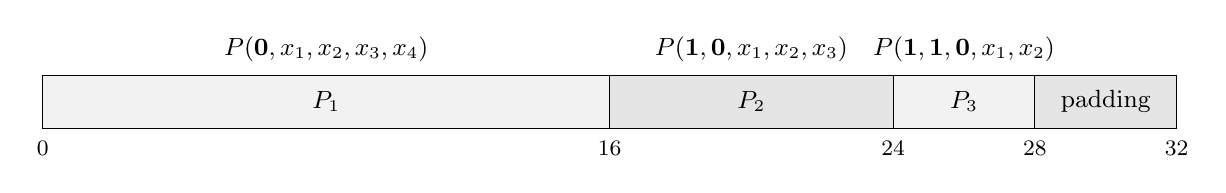
\begin{tikzpicture}[scale=0.45, every node/.style={font=\small}]
    \fill[gray!10] (0,0) rectangle (16,1.5);
    \fill[gray!20] (16,0) rectangle (24,1.5);
    \fill[gray!10] (24,0) rectangle (28,1.5);
    \fill[gray!20] (28,0) rectangle (32,1.5);

    \draw[black] (0,0) rectangle (32,1.5);
    \draw[black] (16,0) -- (16,1.5);
    \draw[black] (24,0) -- (24,1.5);
    \draw[black] (28,0) -- (28,1.5);

    \node at (8,0.75) {$P_1$};
    \node at (20,0.75) {$P_2$};
    \node at (26,0.75) {$P_3$};
    \node at (30,0.75) {padding};

    \node[below] at (0,-0.1) {\footnotesize 0};
    \node[below] at (16,-0.1) {\footnotesize 16};
    \node[below] at (24,-0.1) {\footnotesize 24};
    \node[below] at (28,-0.1) {\footnotesize 28};
    \node[below] at (32,-0.1) {\footnotesize 32};

    % Selector annotations above each section
    \node[above] at (8,1.6) {$P({\mathbf{0}}, x_1, x_2, x_3, x_4)$};
    \node[above] at (20,1.6) {$P({\mathbf{1}}, {\mathbf{0}}, x_1, x_2, x_3)$};
    \node[above] at (26,1.6) {$P({\mathbf{1}}, {\mathbf{1}}, {\mathbf{0}}, x_1, x_2)$};
\end{tikzpicture}
\caption{Simple stacking of $P_1, P_2, P_3$ into a single polynomial $P$}
\label{fig:stacking}
\end{figure}

Advantage of this approach: simplicity.

Drawback: padding overhead, i.e. it does not take advantage of the potential repetions at the end of each inner polynomial's evaluations.

\vspace{5mm}

There are alterntive ways to handle the stacking of multiple multilinear polynomials:

\begin{itemize}
    \item \textbf{Jagged PCS} \cite{jagged_pcs}: No padding overhead, at the cost of an additional sumcheck.
    \item  \textbf{Per-polynomial chunking}: decompose the non-repeated par of each inner polynomial into a small (think 3 or 4) number of power-of-two sized chunks, and concatenate all these chunks into a single large polynomial.
\end{itemize}

\textit{Note 3:} A meticulous implementation of WHIR could also take advantage of any potential repetitions in the committed polynomial, both at the FFT and the sumcheck level, leaving the Merklelisation as the main overhead.

\section{Recursive Aggregation}\label{sec:recursive-aggregation}

The recursive aggregation program (see Figure~\ref{fig:recursive-aggregation}) attests that a set of public keys have valid signatures for a given message. It partitions the signers into $n_{\text{rec}} + 1$ sources: one \textbf{direct source} whose XMSS signatures are verified explicitly, and $n_{\text{rec}} \geq 0$ \textbf{recursive sources}, each accompanied by a sub-proof that is recursively verified.

For each recursive source, the program runs the leanVM verifier on the provided sub-proof, confirming that the sub-proof itself is a valid recursive aggregation proof covering the source's signers. When $n_{\text{rec}} = 0$, the program simply verifies all signatures directly.

\subsection{Bytecode evaluation claims}\label{sec:bytecode-reduction}

A key subtlety arises from recursion. Every leanVM proof is tied to a specific \emph{bytecode} --- the program that was executed, represented as a multilinear polynomial. In our case, there is a single program (that both contain signature verification and recursion algorithms). The leanVM verification algorithm requires evaluating the bytecode polynomial at a random point.

When the recursive aggregation program verifies a sub-proof, it runs the leanVM verifier \emph{inside} the program. This verification produces a bytecode evaluation claim. For efficiency, rather than checking it inside the program (with a PCS), the claim is forwarded to the public input, to be checked externally.

However, each sub-proof is potentially itself a recursive aggregation, and may have already forwarded its own bytecode claim in the same way. So for each of the $n_{\text{rec}}$ sub-proofs, \textbf{two} bytecode claims arise:

\begin{enumerate}
    \item \textbf{Inner-public-memory claim}: The bytecode claim that the sub-proof forwarded from its own recursive verifications (read from the sub-proof's public input).

    \item \textbf{Inner-proof claim}: The new bytecode claim produced by verifying the sub-proof itself.
\end{enumerate}

After verifying all $n_{\text{rec}}$ sub-proofs, a fresh Fiat--Shamir transcript is initialized and fed with all $2 n_{\text{rec}}$ evaluation points and claimed values. This transcript produces a random linear combination challenge, and the $2 n_{\text{rec}}$ claims are then batched into a single one via sumcheck, yielding a reduced claim. This reduced claim is written to the public input for the next level of recursion.

When $n_{\text{rec}} = 0$ (no recursion), the bytecode claim in the public input is set to zero.


\subsection{Signer partitioning}\label{sec:signer-partitioning}

\emph{
In the following, we assume  the message being signed is common to all signers (typically the case at Ethereum's consensus layer), but the scheme can be naturally adapted to distinct messages.}

\vspace{3mm}

Consider an aggregation of $n_{\text{sigs}}$ (distinct) signatures. The $n_{\text{sigs}}$ (distinct) public keys are part of the "public input" in memory. The aggregation program must ensure that each public key is verified by at least one of the $1 + n_{\text{rec}}$ sources (duplications allowed: some public keys may be verified by multiple sources).

Let $n_{\text{dup}}$ be the total number of duplicated public keys across sources, counted with multiplicity. To ensure ensure valid partionning, we use the following algorithm:

\begin{itemize}
    \item Initialize a counter $c \gets 0$.
    \item Initialize a (write-once) array $B$ of size $n_{\text{total}} = n_{\text{sigs}} + n_{\text{dup}}$.
    \item For each source $s$, for each signature index $i \in [0, n_{\text{total}})$ verified by $s$, write $B[i] \gets c$ and increment $c$.
    \item At the end, assert $c = n_{\text{total}}$.
\end{itemize}

\clearpage
\bibliographystyle{IEEEtran}
\bibliography{bibliography}

\end{document}